% Created by tikzDevice version 0.12 on 2019-05-17 13:10:41
% !TEX encoding = UTF-8 Unicode
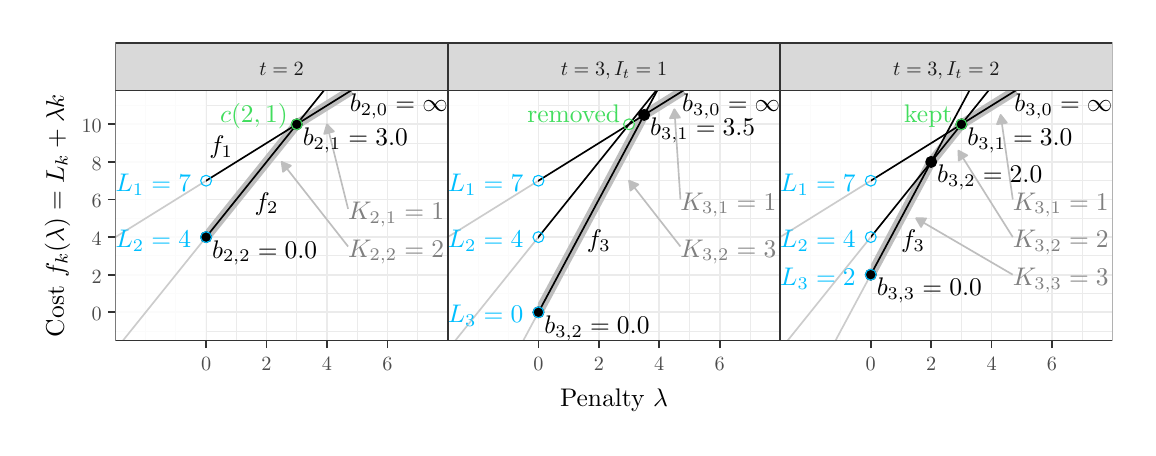
\begin{tikzpicture}[x=1pt,y=1pt]
\definecolor{fillColor}{RGB}{255,255,255}
\path[use as bounding box,fill=fillColor,fill opacity=0.00] (0,0) rectangle (397.48,144.54);
\begin{scope}
\path[clip] (  0.00,  0.00) rectangle (397.48,144.54);
\definecolor{drawColor}{RGB}{255,255,255}
\definecolor{fillColor}{RGB}{255,255,255}

\path[draw=drawColor,line width= 0.6pt,line join=round,line cap=round,fill=fillColor] ( -0.00,  0.00) rectangle (397.48,144.54);
\end{scope}
\begin{scope}
\path[clip] ( 31.72, 31.50) rectangle (151.81,121.85);
\definecolor{fillColor}{RGB}{255,255,255}

\path[fill=fillColor] ( 31.72, 31.50) rectangle (151.81,121.85);
\definecolor{drawColor}{gray}{0.92}

\path[draw=drawColor,line width= 0.3pt,line join=round] ( 31.72, 34.90) --
	(151.81, 34.90);

\path[draw=drawColor,line width= 0.3pt,line join=round] ( 31.72, 48.48) --
	(151.81, 48.48);

\path[draw=drawColor,line width= 0.3pt,line join=round] ( 31.72, 62.07) --
	(151.81, 62.07);

\path[draw=drawColor,line width= 0.3pt,line join=round] ( 31.72, 75.66) --
	(151.81, 75.66);

\path[draw=drawColor,line width= 0.3pt,line join=round] ( 31.72, 89.24) --
	(151.81, 89.24);

\path[draw=drawColor,line width= 0.3pt,line join=round] ( 31.72,102.83) --
	(151.81,102.83);

\path[draw=drawColor,line width= 0.3pt,line join=round] ( 31.72,116.41) --
	(151.81,116.41);

\path[draw=drawColor,line width= 0.3pt,line join=round] ( 42.64, 31.50) --
	( 42.64,121.85);

\path[draw=drawColor,line width= 0.3pt,line join=round] ( 53.56, 31.50) --
	( 53.56,121.85);

\path[draw=drawColor,line width= 0.3pt,line join=round] ( 75.39, 31.50) --
	( 75.39,121.85);

\path[draw=drawColor,line width= 0.3pt,line join=round] ( 97.23, 31.50) --
	( 97.23,121.85);

\path[draw=drawColor,line width= 0.3pt,line join=round] (119.06, 31.50) --
	(119.06,121.85);

\path[draw=drawColor,line width= 0.3pt,line join=round] (140.89, 31.50) --
	(140.89,121.85);

\path[draw=drawColor,line width= 0.3pt,line join=round] (151.81, 31.50) --
	(151.81,121.85);

\path[draw=drawColor,line width= 0.6pt,line join=round] ( 31.72, 41.69) --
	(151.81, 41.69);

\path[draw=drawColor,line width= 0.6pt,line join=round] ( 31.72, 55.28) --
	(151.81, 55.28);

\path[draw=drawColor,line width= 0.6pt,line join=round] ( 31.72, 68.86) --
	(151.81, 68.86);

\path[draw=drawColor,line width= 0.6pt,line join=round] ( 31.72, 82.45) --
	(151.81, 82.45);

\path[draw=drawColor,line width= 0.6pt,line join=round] ( 31.72, 96.03) --
	(151.81, 96.03);

\path[draw=drawColor,line width= 0.6pt,line join=round] ( 31.72,109.62) --
	(151.81,109.62);

\path[draw=drawColor,line width= 0.6pt,line join=round] ( 64.47, 31.50) --
	( 64.47,121.85);

\path[draw=drawColor,line width= 0.6pt,line join=round] ( 86.31, 31.50) --
	( 86.31,121.85);

\path[draw=drawColor,line width= 0.6pt,line join=round] (108.14, 31.50) --
	(108.14,121.85);

\path[draw=drawColor,line width= 0.6pt,line join=round] (129.98, 31.50) --
	(129.98,121.85);
\definecolor{drawColor}{RGB}{190,190,190}

\path[draw=drawColor,line width= 3.4pt,line join=round] ( 64.47, 68.86) --
	( 65.57, 70.22) --
	( 66.66, 71.58) --
	( 67.75, 72.94) --
	( 68.84, 74.30) --
	( 69.93, 75.66) --
	( 71.02, 77.01) --
	( 72.12, 78.37) --
	( 73.21, 79.73) --
	( 74.30, 81.09) --
	( 75.39, 82.45) --
	( 76.48, 83.81) --
	( 77.57, 85.17) --
	( 78.67, 86.52) --
	( 79.76, 87.88) --
	( 80.85, 89.24) --
	( 81.94, 90.60) --
	( 83.03, 91.96) --
	( 84.12, 93.32) --
	( 85.22, 94.68) --
	( 86.31, 96.03) --
	( 87.40, 97.39) --
	( 88.49, 98.75) --
	( 89.58,100.11) --
	( 90.68,101.47) --
	( 91.77,102.83) --
	( 92.86,104.19) --
	( 93.95,105.54) --
	( 95.04,106.90) --
	( 96.13,108.26) --
	( 97.23,109.62) --
	( 98.32,110.30) --
	( 99.41,110.98) --
	(100.50,111.66) --
	(101.59,112.34) --
	(102.68,113.02) --
	(103.78,113.70) --
	(104.87,114.37) --
	(105.96,115.05) --
	(107.05,115.73) --
	(108.14,116.41) --
	(109.23,117.09) --
	(110.33,117.77) --
	(111.42,118.45) --
	(112.51,119.13) --
	(113.60,119.81) --
	(114.69,120.49) --
	(115.78,121.17) --
	(116.88,121.85);

\path[draw=drawColor,line width= 0.6pt,line join=round] (115.78, 79.05) -- (108.14,109.62);
\definecolor{fillColor}{RGB}{190,190,190}

\path[draw=drawColor,line width= 0.6pt,line join=round,fill=fillColor] (110.65,107.02) --
	(108.14,109.62) --
	(107.15,106.15) --
	cycle;

\path[draw=drawColor,line width= 0.6pt,line join=round] (115.78, 65.47) -- ( 91.77, 96.03);

\path[draw=drawColor,line width= 0.6pt,line join=round,fill=fillColor] ( 95.12, 94.69) --
	( 91.77, 96.03) --
	( 92.28, 92.46) --
	cycle;
\definecolor{drawColor}{RGB}{0,0,0}

\node[text=drawColor,anchor=base west,inner sep=0pt, outer sep=0pt, scale=  0.92] at ( 66.66, 61.26) {$b_{2,2}=0.0$};

\node[text=drawColor,anchor=base west,inner sep=0pt, outer sep=0pt, scale=  0.92] at ( 99.41,102.02) {$b_{2,1}=3.0$};

\path[draw=drawColor,line width= 0.6pt,line join=round] ( 31.72, 68.86) -- (151.81,143.58);

\path[draw=drawColor,line width= 0.6pt,line join=round] ( 31.72, 28.11) -- (125.29,144.54);
\definecolor{fillColor}{RGB}{255,255,255}

\path[fill=fillColor,fill opacity=0.80] ( 31.72, 31.50) rectangle ( 64.47,121.85);
\definecolor{drawColor}{gray}{0.50}

\node[text=drawColor,anchor=base west,inner sep=0pt, outer sep=0pt, scale=  0.92] at (115.78, 75.25) {$K_{2,1}=1$};

\node[text=drawColor,anchor=base west,inner sep=0pt, outer sep=0pt, scale=  0.92] at (115.78, 61.66) {$K_{2,2}=2$};
\definecolor{drawColor}{RGB}{0,0,0}
\definecolor{fillColor}{RGB}{0,0,0}

\path[draw=drawColor,line width= 0.4pt,line join=round,line cap=round,fill=fillColor] ( 64.47, 68.86) circle (  1.96);

\path[draw=drawColor,line width= 0.4pt,line join=round,line cap=round,fill=fillColor] ( 97.23,109.62) circle (  1.96);
\definecolor{drawColor}{RGB}{65,221,93}

\path[draw=drawColor,line width= 0.4pt,line join=round,line cap=round] ( 97.23,109.62) circle (  1.96);

\node[text=drawColor,anchor=base east,inner sep=0pt, outer sep=0pt, scale=  0.92] at ( 93.95,110.30) {$c(2, 1)$};
\definecolor{drawColor}{RGB}{0,0,0}

\node[text=drawColor,anchor=base,inner sep=0pt, outer sep=0pt, scale=  0.92] at ( 69.93, 99.03) {$f_1$};

\node[text=drawColor,anchor=base,inner sep=0pt, outer sep=0pt, scale=  0.92] at ( 86.31, 78.65) {$f_2$};

\node[text=drawColor,anchor=base east,inner sep=0pt, outer sep=0pt, scale=  0.92] at (151.81,114.24) {$b_{2,0}=\infty$};
\definecolor{drawColor}{RGB}{0,191,255}

\node[text=drawColor,anchor=base east,inner sep=0pt, outer sep=0pt, scale=  0.92] at ( 59.02, 85.44) {$L_1=7$};

\node[text=drawColor,anchor=base east,inner sep=0pt, outer sep=0pt, scale=  0.92] at ( 59.02, 65.06) {$L_2=4$};

\path[draw=drawColor,line width= 0.4pt,line join=round,line cap=round] ( 64.47, 89.24) circle (  1.96);

\path[draw=drawColor,line width= 0.4pt,line join=round,line cap=round] ( 64.47, 68.86) circle (  1.96);
\definecolor{drawColor}{gray}{0.20}

\path[draw=drawColor,line width= 0.6pt,line join=round,line cap=round] ( 31.72, 31.50) rectangle (151.81,121.85);
\end{scope}
\begin{scope}
\path[clip] (151.81, 31.50) rectangle (271.90,121.85);
\definecolor{fillColor}{RGB}{255,255,255}

\path[fill=fillColor] (151.81, 31.50) rectangle (271.90,121.85);
\definecolor{drawColor}{gray}{0.92}

\path[draw=drawColor,line width= 0.3pt,line join=round] (151.81, 34.90) --
	(271.90, 34.90);

\path[draw=drawColor,line width= 0.3pt,line join=round] (151.81, 48.48) --
	(271.90, 48.48);

\path[draw=drawColor,line width= 0.3pt,line join=round] (151.81, 62.07) --
	(271.90, 62.07);

\path[draw=drawColor,line width= 0.3pt,line join=round] (151.81, 75.66) --
	(271.90, 75.66);

\path[draw=drawColor,line width= 0.3pt,line join=round] (151.81, 89.24) --
	(271.90, 89.24);

\path[draw=drawColor,line width= 0.3pt,line join=round] (151.81,102.83) --
	(271.90,102.83);

\path[draw=drawColor,line width= 0.3pt,line join=round] (151.81,116.41) --
	(271.90,116.41);

\path[draw=drawColor,line width= 0.3pt,line join=round] (162.73, 31.50) --
	(162.73,121.85);

\path[draw=drawColor,line width= 0.3pt,line join=round] (173.64, 31.50) --
	(173.64,121.85);

\path[draw=drawColor,line width= 0.3pt,line join=round] (195.48, 31.50) --
	(195.48,121.85);

\path[draw=drawColor,line width= 0.3pt,line join=round] (217.31, 31.50) --
	(217.31,121.85);

\path[draw=drawColor,line width= 0.3pt,line join=round] (239.15, 31.50) --
	(239.15,121.85);

\path[draw=drawColor,line width= 0.3pt,line join=round] (260.98, 31.50) --
	(260.98,121.85);

\path[draw=drawColor,line width= 0.3pt,line join=round] (271.90, 31.50) --
	(271.90,121.85);

\path[draw=drawColor,line width= 0.6pt,line join=round] (151.81, 41.69) --
	(271.90, 41.69);

\path[draw=drawColor,line width= 0.6pt,line join=round] (151.81, 55.28) --
	(271.90, 55.28);

\path[draw=drawColor,line width= 0.6pt,line join=round] (151.81, 68.86) --
	(271.90, 68.86);

\path[draw=drawColor,line width= 0.6pt,line join=round] (151.81, 82.45) --
	(271.90, 82.45);

\path[draw=drawColor,line width= 0.6pt,line join=round] (151.81, 96.03) --
	(271.90, 96.03);

\path[draw=drawColor,line width= 0.6pt,line join=round] (151.81,109.62) --
	(271.90,109.62);

\path[draw=drawColor,line width= 0.6pt,line join=round] (184.56, 31.50) --
	(184.56,121.85);

\path[draw=drawColor,line width= 0.6pt,line join=round] (206.40, 31.50) --
	(206.40,121.85);

\path[draw=drawColor,line width= 0.6pt,line join=round] (228.23, 31.50) --
	(228.23,121.85);

\path[draw=drawColor,line width= 0.6pt,line join=round] (250.06, 31.50) --
	(250.06,121.85);
\definecolor{drawColor}{RGB}{190,190,190}

\path[draw=drawColor,line width= 3.4pt,line join=round] (184.56, 41.69) --
	(185.65, 43.73) --
	(186.74, 45.77) --
	(187.84, 47.81) --
	(188.93, 49.84) --
	(190.02, 51.88) --
	(191.11, 53.92) --
	(192.20, 55.96) --
	(193.30, 57.99) --
	(194.39, 60.03) --
	(195.48, 62.07) --
	(196.57, 64.11) --
	(197.66, 66.15) --
	(198.75, 68.18) --
	(199.85, 70.22) --
	(200.94, 72.26) --
	(202.03, 74.30) --
	(203.12, 76.33) --
	(204.21, 78.37) --
	(205.30, 80.41) --
	(206.40, 82.45) --
	(207.49, 84.49) --
	(208.58, 86.52) --
	(209.67, 88.56) --
	(210.76, 90.60) --
	(211.85, 92.64) --
	(212.95, 94.68) --
	(214.04, 96.71) --
	(215.13, 98.75) --
	(216.22,100.79) --
	(217.31,102.83) --
	(218.40,104.86) --
	(219.50,106.90) --
	(220.59,108.94) --
	(221.68,110.98) --
	(222.77,113.02) --
	(223.86,113.70) --
	(224.95,114.37) --
	(226.05,115.05) --
	(227.14,115.73) --
	(228.23,116.41) --
	(229.32,117.09) --
	(230.41,117.77) --
	(231.50,118.45) --
	(232.60,119.13) --
	(233.69,119.81) --
	(234.78,120.49) --
	(235.87,121.17) --
	(236.96,121.85);

\path[draw=drawColor,line width= 0.6pt,line join=round] (235.87, 82.45) -- (233.69,115.05);
\definecolor{fillColor}{RGB}{190,190,190}

\path[draw=drawColor,line width= 0.6pt,line join=round,fill=fillColor] (235.70,112.05) --
	(233.69,115.05) --
	(232.09,111.81) --
	cycle;

\path[draw=drawColor,line width= 0.6pt,line join=round] (235.87, 65.47) -- (217.31, 89.24);

\path[draw=drawColor,line width= 0.6pt,line join=round,fill=fillColor] (220.66, 87.89) --
	(217.31, 89.24) --
	(217.81, 85.66) --
	cycle;
\definecolor{drawColor}{RGB}{0,0,0}

\node[text=drawColor,anchor=base west,inner sep=0pt, outer sep=0pt, scale=  0.92] at (186.74, 34.09) {$b_{3,2}=0.0$};

\node[text=drawColor,anchor=base west,inner sep=0pt, outer sep=0pt, scale=  0.92] at (224.95,105.41) {$b_{3,1}=3.5$};

\path[draw=drawColor,line width= 0.6pt,line join=round] (151.81, 68.86) -- (271.90,143.58);

\path[draw=drawColor,line width= 0.6pt,line join=round] (151.81, 28.11) -- (245.37,144.54);

\path[draw=drawColor,line width= 0.6pt,line join=round] (162.23,  0.00) -- (239.66,144.54);
\definecolor{fillColor}{RGB}{255,255,255}

\path[fill=fillColor,fill opacity=0.80] (151.81, 31.50) rectangle (184.56,121.85);
\definecolor{drawColor}{gray}{0.50}

\node[text=drawColor,anchor=base west,inner sep=0pt, outer sep=0pt, scale=  0.92] at (235.87, 78.65) {$K_{3,1}=1$};

\node[text=drawColor,anchor=base west,inner sep=0pt, outer sep=0pt, scale=  0.92] at (235.87, 61.66) {$K_{3,2}=3$};
\definecolor{drawColor}{RGB}{0,0,0}
\definecolor{fillColor}{RGB}{0,0,0}

\path[draw=drawColor,line width= 0.4pt,line join=round,line cap=round,fill=fillColor] (184.56, 41.69) circle (  1.96);

\path[draw=drawColor,line width= 0.4pt,line join=round,line cap=round,fill=fillColor] (222.77,113.02) circle (  1.96);
\definecolor{drawColor}{RGB}{65,221,93}

\path[draw=drawColor,line width= 0.4pt,line join=round,line cap=round] (217.31,109.62) circle (  1.96);

\node[text=drawColor,anchor=base east,inner sep=0pt, outer sep=0pt, scale=  0.92] at (214.04,110.30) {removed};
\definecolor{drawColor}{RGB}{0,0,0}

\node[text=drawColor,anchor=base,inner sep=0pt, outer sep=0pt, scale=  0.92] at (206.40, 65.06) {$f_3$};

\node[text=drawColor,anchor=base east,inner sep=0pt, outer sep=0pt, scale=  0.92] at (271.90,114.24) {$b_{3,0}=\infty$};
\definecolor{drawColor}{RGB}{0,191,255}

\node[text=drawColor,anchor=base east,inner sep=0pt, outer sep=0pt, scale=  0.92] at (179.10, 85.44) {$L_1=7$};

\node[text=drawColor,anchor=base east,inner sep=0pt, outer sep=0pt, scale=  0.92] at (179.10, 65.06) {$L_2=4$};

\node[text=drawColor,anchor=base east,inner sep=0pt, outer sep=0pt, scale=  0.92] at (179.10, 37.89) {$L_3=0$};

\path[draw=drawColor,line width= 0.4pt,line join=round,line cap=round] (184.56, 89.24) circle (  1.96);

\path[draw=drawColor,line width= 0.4pt,line join=round,line cap=round] (184.56, 68.86) circle (  1.96);

\path[draw=drawColor,line width= 0.4pt,line join=round,line cap=round] (184.56, 41.69) circle (  1.96);
\definecolor{drawColor}{gray}{0.20}

\path[draw=drawColor,line width= 0.6pt,line join=round,line cap=round] (151.81, 31.50) rectangle (271.90,121.85);
\end{scope}
\begin{scope}
\path[clip] (271.90, 31.50) rectangle (391.98,121.85);
\definecolor{fillColor}{RGB}{255,255,255}

\path[fill=fillColor] (271.90, 31.50) rectangle (391.98,121.85);
\definecolor{drawColor}{gray}{0.92}

\path[draw=drawColor,line width= 0.3pt,line join=round] (271.90, 34.90) --
	(391.98, 34.90);

\path[draw=drawColor,line width= 0.3pt,line join=round] (271.90, 48.48) --
	(391.98, 48.48);

\path[draw=drawColor,line width= 0.3pt,line join=round] (271.90, 62.07) --
	(391.98, 62.07);

\path[draw=drawColor,line width= 0.3pt,line join=round] (271.90, 75.66) --
	(391.98, 75.66);

\path[draw=drawColor,line width= 0.3pt,line join=round] (271.90, 89.24) --
	(391.98, 89.24);

\path[draw=drawColor,line width= 0.3pt,line join=round] (271.90,102.83) --
	(391.98,102.83);

\path[draw=drawColor,line width= 0.3pt,line join=round] (271.90,116.41) --
	(391.98,116.41);

\path[draw=drawColor,line width= 0.3pt,line join=round] (282.81, 31.50) --
	(282.81,121.85);

\path[draw=drawColor,line width= 0.3pt,line join=round] (293.73, 31.50) --
	(293.73,121.85);

\path[draw=drawColor,line width= 0.3pt,line join=round] (315.57, 31.50) --
	(315.57,121.85);

\path[draw=drawColor,line width= 0.3pt,line join=round] (337.40, 31.50) --
	(337.40,121.85);

\path[draw=drawColor,line width= 0.3pt,line join=round] (359.23, 31.50) --
	(359.23,121.85);

\path[draw=drawColor,line width= 0.3pt,line join=round] (381.07, 31.50) --
	(381.07,121.85);

\path[draw=drawColor,line width= 0.3pt,line join=round] (391.98, 31.50) --
	(391.98,121.85);

\path[draw=drawColor,line width= 0.6pt,line join=round] (271.90, 41.69) --
	(391.98, 41.69);

\path[draw=drawColor,line width= 0.6pt,line join=round] (271.90, 55.28) --
	(391.98, 55.28);

\path[draw=drawColor,line width= 0.6pt,line join=round] (271.90, 68.86) --
	(391.98, 68.86);

\path[draw=drawColor,line width= 0.6pt,line join=round] (271.90, 82.45) --
	(391.98, 82.45);

\path[draw=drawColor,line width= 0.6pt,line join=round] (271.90, 96.03) --
	(391.98, 96.03);

\path[draw=drawColor,line width= 0.6pt,line join=round] (271.90,109.62) --
	(391.98,109.62);

\path[draw=drawColor,line width= 0.6pt,line join=round] (304.65, 31.50) --
	(304.65,121.85);

\path[draw=drawColor,line width= 0.6pt,line join=round] (326.48, 31.50) --
	(326.48,121.85);

\path[draw=drawColor,line width= 0.6pt,line join=round] (348.32, 31.50) --
	(348.32,121.85);

\path[draw=drawColor,line width= 0.6pt,line join=round] (370.15, 31.50) --
	(370.15,121.85);
\definecolor{drawColor}{RGB}{190,190,190}

\path[draw=drawColor,line width= 3.4pt,line join=round] (304.65, 55.28) --
	(305.74, 57.31) --
	(306.83, 59.35) --
	(307.92, 61.39) --
	(309.02, 63.43) --
	(310.11, 65.47) --
	(311.20, 67.50) --
	(312.29, 69.54) --
	(313.38, 71.58) --
	(314.47, 73.62) --
	(315.57, 75.66) --
	(316.66, 77.69) --
	(317.75, 79.73) --
	(318.84, 81.77) --
	(319.93, 83.81) --
	(321.02, 85.84) --
	(322.12, 87.88) --
	(323.21, 89.92) --
	(324.30, 91.96) --
	(325.39, 94.00) --
	(326.48, 96.03) --
	(327.57, 97.39) --
	(328.67, 98.75) --
	(329.76,100.11) --
	(330.85,101.47) --
	(331.94,102.83) --
	(333.03,104.19) --
	(334.12,105.54) --
	(335.22,106.90) --
	(336.31,108.26) --
	(337.40,109.62) --
	(338.49,110.30) --
	(339.58,110.98) --
	(340.67,111.66) --
	(341.77,112.34) --
	(342.86,113.02) --
	(343.95,113.70) --
	(345.04,114.37) --
	(346.13,115.05) --
	(347.23,115.73) --
	(348.32,116.41) --
	(349.41,117.09) --
	(350.50,117.77) --
	(351.59,118.45) --
	(352.68,119.13) --
	(353.78,119.81) --
	(354.87,120.49) --
	(355.96,121.17) --
	(357.05,121.85);

\path[draw=drawColor,line width= 0.6pt,line join=round] (355.96, 82.45) -- (351.59,113.02);
\definecolor{fillColor}{RGB}{190,190,190}

\path[draw=drawColor,line width= 0.6pt,line join=round,fill=fillColor] (353.82,110.17) --
	(351.59,113.02) --
	(350.25,109.66) --
	cycle;

\path[draw=drawColor,line width= 0.6pt,line join=round] (355.96, 68.86) -- (336.31,100.11);

\path[draw=drawColor,line width= 0.6pt,line join=round,fill=fillColor] (339.50, 98.42) --
	(336.31,100.11) --
	(336.44, 96.50) --
	cycle;

\path[draw=drawColor,line width= 0.6pt,line join=round] (355.96, 55.28) -- (321.02, 75.66);

\path[draw=drawColor,line width= 0.6pt,line join=round,fill=fillColor] (324.64, 75.64) --
	(321.02, 75.66) --
	(322.82, 72.52) --
	cycle;
\definecolor{drawColor}{RGB}{0,0,0}

\node[text=drawColor,anchor=base west,inner sep=0pt, outer sep=0pt, scale=  0.92] at (306.83, 47.67) {$b_{3,3}=0.0$};

\node[text=drawColor,anchor=base west,inner sep=0pt, outer sep=0pt, scale=  0.92] at (328.67, 88.43) {$b_{3,2}=2.0$};

\node[text=drawColor,anchor=base west,inner sep=0pt, outer sep=0pt, scale=  0.92] at (339.58,102.02) {$b_{3,1}=3.0$};

\path[draw=drawColor,line width= 0.6pt,line join=round] (271.90, 68.86) -- (391.98,143.58);

\path[draw=drawColor,line width= 0.6pt,line join=round] (271.90, 28.11) -- (365.46,144.54);

\path[draw=drawColor,line width= 0.6pt,line join=round] (275.04,  0.00) -- (352.47,144.54);
\definecolor{fillColor}{RGB}{255,255,255}

\path[fill=fillColor,fill opacity=0.80] (271.90, 31.50) rectangle (304.65,121.85);
\definecolor{drawColor}{gray}{0.50}

\node[text=drawColor,anchor=base west,inner sep=0pt, outer sep=0pt, scale=  0.92] at (355.96, 78.65) {$K_{3,1}=1$};

\node[text=drawColor,anchor=base west,inner sep=0pt, outer sep=0pt, scale=  0.92] at (355.96, 65.06) {$K_{3,2}=2$};

\node[text=drawColor,anchor=base west,inner sep=0pt, outer sep=0pt, scale=  0.92] at (355.96, 51.48) {$K_{3,3}=3$};
\definecolor{drawColor}{RGB}{0,0,0}
\definecolor{fillColor}{RGB}{0,0,0}

\path[draw=drawColor,line width= 0.4pt,line join=round,line cap=round,fill=fillColor] (304.65, 55.28) circle (  1.96);

\path[draw=drawColor,line width= 0.4pt,line join=round,line cap=round,fill=fillColor] (326.48, 96.03) circle (  1.96);

\path[draw=drawColor,line width= 0.4pt,line join=round,line cap=round,fill=fillColor] (337.40,109.62) circle (  1.96);
\definecolor{drawColor}{RGB}{65,221,93}

\path[draw=drawColor,line width= 0.4pt,line join=round,line cap=round] (337.40,109.62) circle (  1.96);

\node[text=drawColor,anchor=base east,inner sep=0pt, outer sep=0pt, scale=  0.92] at (334.12,110.30) {kept};
\definecolor{drawColor}{RGB}{0,0,0}

\node[text=drawColor,anchor=base,inner sep=0pt, outer sep=0pt, scale=  0.92] at (319.93, 65.06) {$f_3$};

\node[text=drawColor,anchor=base east,inner sep=0pt, outer sep=0pt, scale=  0.92] at (391.98,114.24) {$b_{3,0}=\infty$};
\definecolor{drawColor}{RGB}{0,191,255}

\node[text=drawColor,anchor=base east,inner sep=0pt, outer sep=0pt, scale=  0.92] at (299.19, 85.44) {$L_1=7$};

\node[text=drawColor,anchor=base east,inner sep=0pt, outer sep=0pt, scale=  0.92] at (299.19, 65.06) {$L_2=4$};

\node[text=drawColor,anchor=base east,inner sep=0pt, outer sep=0pt, scale=  0.92] at (299.19, 51.48) {$L_3=2$};

\path[draw=drawColor,line width= 0.4pt,line join=round,line cap=round] (304.65, 89.24) circle (  1.96);

\path[draw=drawColor,line width= 0.4pt,line join=round,line cap=round] (304.65, 68.86) circle (  1.96);

\path[draw=drawColor,line width= 0.4pt,line join=round,line cap=round] (304.65, 55.28) circle (  1.96);
\definecolor{drawColor}{gray}{0.20}

\path[draw=drawColor,line width= 0.6pt,line join=round,line cap=round] (271.90, 31.50) rectangle (391.98,121.85);
\end{scope}
\begin{scope}
\path[clip] ( 31.72,121.85) rectangle (151.81,139.04);
\definecolor{drawColor}{gray}{0.20}
\definecolor{fillColor}{gray}{0.85}

\path[draw=drawColor,line width= 0.6pt,line join=round,line cap=round,fill=fillColor] ( 31.72,121.85) rectangle (151.81,139.04);
\definecolor{drawColor}{gray}{0.10}

\node[text=drawColor,anchor=base,inner sep=0pt, outer sep=0pt, scale=  0.73] at ( 91.77,127.41) {$t=2$};
\end{scope}
\begin{scope}
\path[clip] (151.81,121.85) rectangle (271.90,139.04);
\definecolor{drawColor}{gray}{0.20}
\definecolor{fillColor}{gray}{0.85}

\path[draw=drawColor,line width= 0.6pt,line join=round,line cap=round,fill=fillColor] (151.81,121.85) rectangle (271.90,139.04);
\definecolor{drawColor}{gray}{0.10}

\node[text=drawColor,anchor=base,inner sep=0pt, outer sep=0pt, scale=  0.73] at (211.85,127.41) {$t=3, I_t=1$};
\end{scope}
\begin{scope}
\path[clip] (271.90,121.85) rectangle (391.98,139.04);
\definecolor{drawColor}{gray}{0.20}
\definecolor{fillColor}{gray}{0.85}

\path[draw=drawColor,line width= 0.6pt,line join=round,line cap=round,fill=fillColor] (271.90,121.85) rectangle (391.98,139.04);
\definecolor{drawColor}{gray}{0.10}

\node[text=drawColor,anchor=base,inner sep=0pt, outer sep=0pt, scale=  0.73] at (331.94,127.41) {$t=3, I_t=2$};
\end{scope}
\begin{scope}
\path[clip] (  0.00,  0.00) rectangle (397.48,144.54);
\definecolor{drawColor}{gray}{0.20}

\path[draw=drawColor,line width= 0.6pt,line join=round] ( 64.47, 28.75) --
	( 64.47, 31.50);

\path[draw=drawColor,line width= 0.6pt,line join=round] ( 86.31, 28.75) --
	( 86.31, 31.50);

\path[draw=drawColor,line width= 0.6pt,line join=round] (108.14, 28.75) --
	(108.14, 31.50);

\path[draw=drawColor,line width= 0.6pt,line join=round] (129.98, 28.75) --
	(129.98, 31.50);
\end{scope}
\begin{scope}
\path[clip] (  0.00,  0.00) rectangle (397.48,144.54);
\definecolor{drawColor}{gray}{0.30}

\node[text=drawColor,anchor=base,inner sep=0pt, outer sep=0pt, scale=  0.73] at ( 64.47, 20.49) {0};

\node[text=drawColor,anchor=base,inner sep=0pt, outer sep=0pt, scale=  0.73] at ( 86.31, 20.49) {2};

\node[text=drawColor,anchor=base,inner sep=0pt, outer sep=0pt, scale=  0.73] at (108.14, 20.49) {4};

\node[text=drawColor,anchor=base,inner sep=0pt, outer sep=0pt, scale=  0.73] at (129.98, 20.49) {6};
\end{scope}
\begin{scope}
\path[clip] (  0.00,  0.00) rectangle (397.48,144.54);
\definecolor{drawColor}{gray}{0.20}

\path[draw=drawColor,line width= 0.6pt,line join=round] (184.56, 28.75) --
	(184.56, 31.50);

\path[draw=drawColor,line width= 0.6pt,line join=round] (206.40, 28.75) --
	(206.40, 31.50);

\path[draw=drawColor,line width= 0.6pt,line join=round] (228.23, 28.75) --
	(228.23, 31.50);

\path[draw=drawColor,line width= 0.6pt,line join=round] (250.06, 28.75) --
	(250.06, 31.50);
\end{scope}
\begin{scope}
\path[clip] (  0.00,  0.00) rectangle (397.48,144.54);
\definecolor{drawColor}{gray}{0.30}

\node[text=drawColor,anchor=base,inner sep=0pt, outer sep=0pt, scale=  0.73] at (184.56, 20.49) {0};

\node[text=drawColor,anchor=base,inner sep=0pt, outer sep=0pt, scale=  0.73] at (206.40, 20.49) {2};

\node[text=drawColor,anchor=base,inner sep=0pt, outer sep=0pt, scale=  0.73] at (228.23, 20.49) {4};

\node[text=drawColor,anchor=base,inner sep=0pt, outer sep=0pt, scale=  0.73] at (250.06, 20.49) {6};
\end{scope}
\begin{scope}
\path[clip] (  0.00,  0.00) rectangle (397.48,144.54);
\definecolor{drawColor}{gray}{0.20}

\path[draw=drawColor,line width= 0.6pt,line join=round] (304.65, 28.75) --
	(304.65, 31.50);

\path[draw=drawColor,line width= 0.6pt,line join=round] (326.48, 28.75) --
	(326.48, 31.50);

\path[draw=drawColor,line width= 0.6pt,line join=round] (348.32, 28.75) --
	(348.32, 31.50);

\path[draw=drawColor,line width= 0.6pt,line join=round] (370.15, 28.75) --
	(370.15, 31.50);
\end{scope}
\begin{scope}
\path[clip] (  0.00,  0.00) rectangle (397.48,144.54);
\definecolor{drawColor}{gray}{0.30}

\node[text=drawColor,anchor=base,inner sep=0pt, outer sep=0pt, scale=  0.73] at (304.65, 20.49) {0};

\node[text=drawColor,anchor=base,inner sep=0pt, outer sep=0pt, scale=  0.73] at (326.48, 20.49) {2};

\node[text=drawColor,anchor=base,inner sep=0pt, outer sep=0pt, scale=  0.73] at (348.32, 20.49) {4};

\node[text=drawColor,anchor=base,inner sep=0pt, outer sep=0pt, scale=  0.73] at (370.15, 20.49) {6};
\end{scope}
\begin{scope}
\path[clip] (  0.00,  0.00) rectangle (397.48,144.54);
\definecolor{drawColor}{gray}{0.30}

\node[text=drawColor,anchor=base east,inner sep=0pt, outer sep=0pt, scale=  0.73] at ( 26.77, 38.66) {0};

\node[text=drawColor,anchor=base east,inner sep=0pt, outer sep=0pt, scale=  0.73] at ( 26.77, 52.25) {2};

\node[text=drawColor,anchor=base east,inner sep=0pt, outer sep=0pt, scale=  0.73] at ( 26.77, 65.83) {4};

\node[text=drawColor,anchor=base east,inner sep=0pt, outer sep=0pt, scale=  0.73] at ( 26.77, 79.42) {6};

\node[text=drawColor,anchor=base east,inner sep=0pt, outer sep=0pt, scale=  0.73] at ( 26.77, 93.00) {8};

\node[text=drawColor,anchor=base east,inner sep=0pt, outer sep=0pt, scale=  0.73] at ( 26.77,106.59) {10};
\end{scope}
\begin{scope}
\path[clip] (  0.00,  0.00) rectangle (397.48,144.54);
\definecolor{drawColor}{gray}{0.20}

\path[draw=drawColor,line width= 0.6pt,line join=round] ( 28.97, 41.69) --
	( 31.72, 41.69);

\path[draw=drawColor,line width= 0.6pt,line join=round] ( 28.97, 55.28) --
	( 31.72, 55.28);

\path[draw=drawColor,line width= 0.6pt,line join=round] ( 28.97, 68.86) --
	( 31.72, 68.86);

\path[draw=drawColor,line width= 0.6pt,line join=round] ( 28.97, 82.45) --
	( 31.72, 82.45);

\path[draw=drawColor,line width= 0.6pt,line join=round] ( 28.97, 96.03) --
	( 31.72, 96.03);

\path[draw=drawColor,line width= 0.6pt,line join=round] ( 28.97,109.62) --
	( 31.72,109.62);
\end{scope}
\begin{scope}
\path[clip] (  0.00,  0.00) rectangle (397.48,144.54);
\definecolor{drawColor}{RGB}{0,0,0}

\node[text=drawColor,anchor=base,inner sep=0pt, outer sep=0pt, scale=  0.92] at (211.85,  7.83) {Penalty $\lambda$};
\end{scope}
\begin{scope}
\path[clip] (  0.00,  0.00) rectangle (397.48,144.54);
\definecolor{drawColor}{RGB}{0,0,0}

\node[text=drawColor,rotate= 90.00,anchor=base,inner sep=0pt, outer sep=0pt, scale=  0.92] at ( 13.08, 76.67) {Cost $f_k(\lambda) = L_k + \lambda k$};
\end{scope}
\end{tikzpicture}
